\documentclass[12pt,aspectratio=169,xcolor=dvipsnames]{beamer}
\usetheme{SimplePlus}
\usepackage{booktabs}
\usepackage{tikz}
\usepackage{pgfplots}
\usepackage{mathtools}

\newcommand{\R}{\mathbb{R}}
\newcommand{\N}{\mathbb{N}}

\title[short title]{Clase 14 Análisis de señales}
\subtitle{}
\author[NA Barnafi] {Nicolás Alejandro Barnafi Wittwer}
\institute[UC|CMM] 
{
    Pontificia Universidad Católica de Chile \\
    Centro de Modelamiento Matemático
}

\titlegraphic{
    \vspace{-1.8cm}
    \begin{flushright}
      
\includegraphics[height=2.5cm]{../images/puc.png} 
    \end{flushright}
}

\date{05/05/2025}
%\setbeamercovered{transparent}

\begin{document}
%%%%%%%%%%%%%%%%%%%%%%%%%%%%%%%%%%%%%%%%%%%%%%%%%%%%%%%
\begin{frame}
    \maketitle
\end{frame}
%%%%%%%%%%%%%%%%%%%%%%%%%%%%%%%%%%%%%%%%%%%%%%%%%%%%%%%
\begin{frame}{Clase de hoy}
    \begin{itemize}
        \item Señales
        \item Espacios de Hilbert y sus propiedades
        \item Ejemplos numéricos
    \end{itemize}

    \vspace{1cm}
    \newref{Curso análisis de Fourier}
\end{frame}
%%%%%%%%%%%%%%%%%%%%%%%%%%%%%%%%%%%%%%%%%%%%%%%%%%%%%%%
\begin{frame}{Señales}
    \begin{center}
        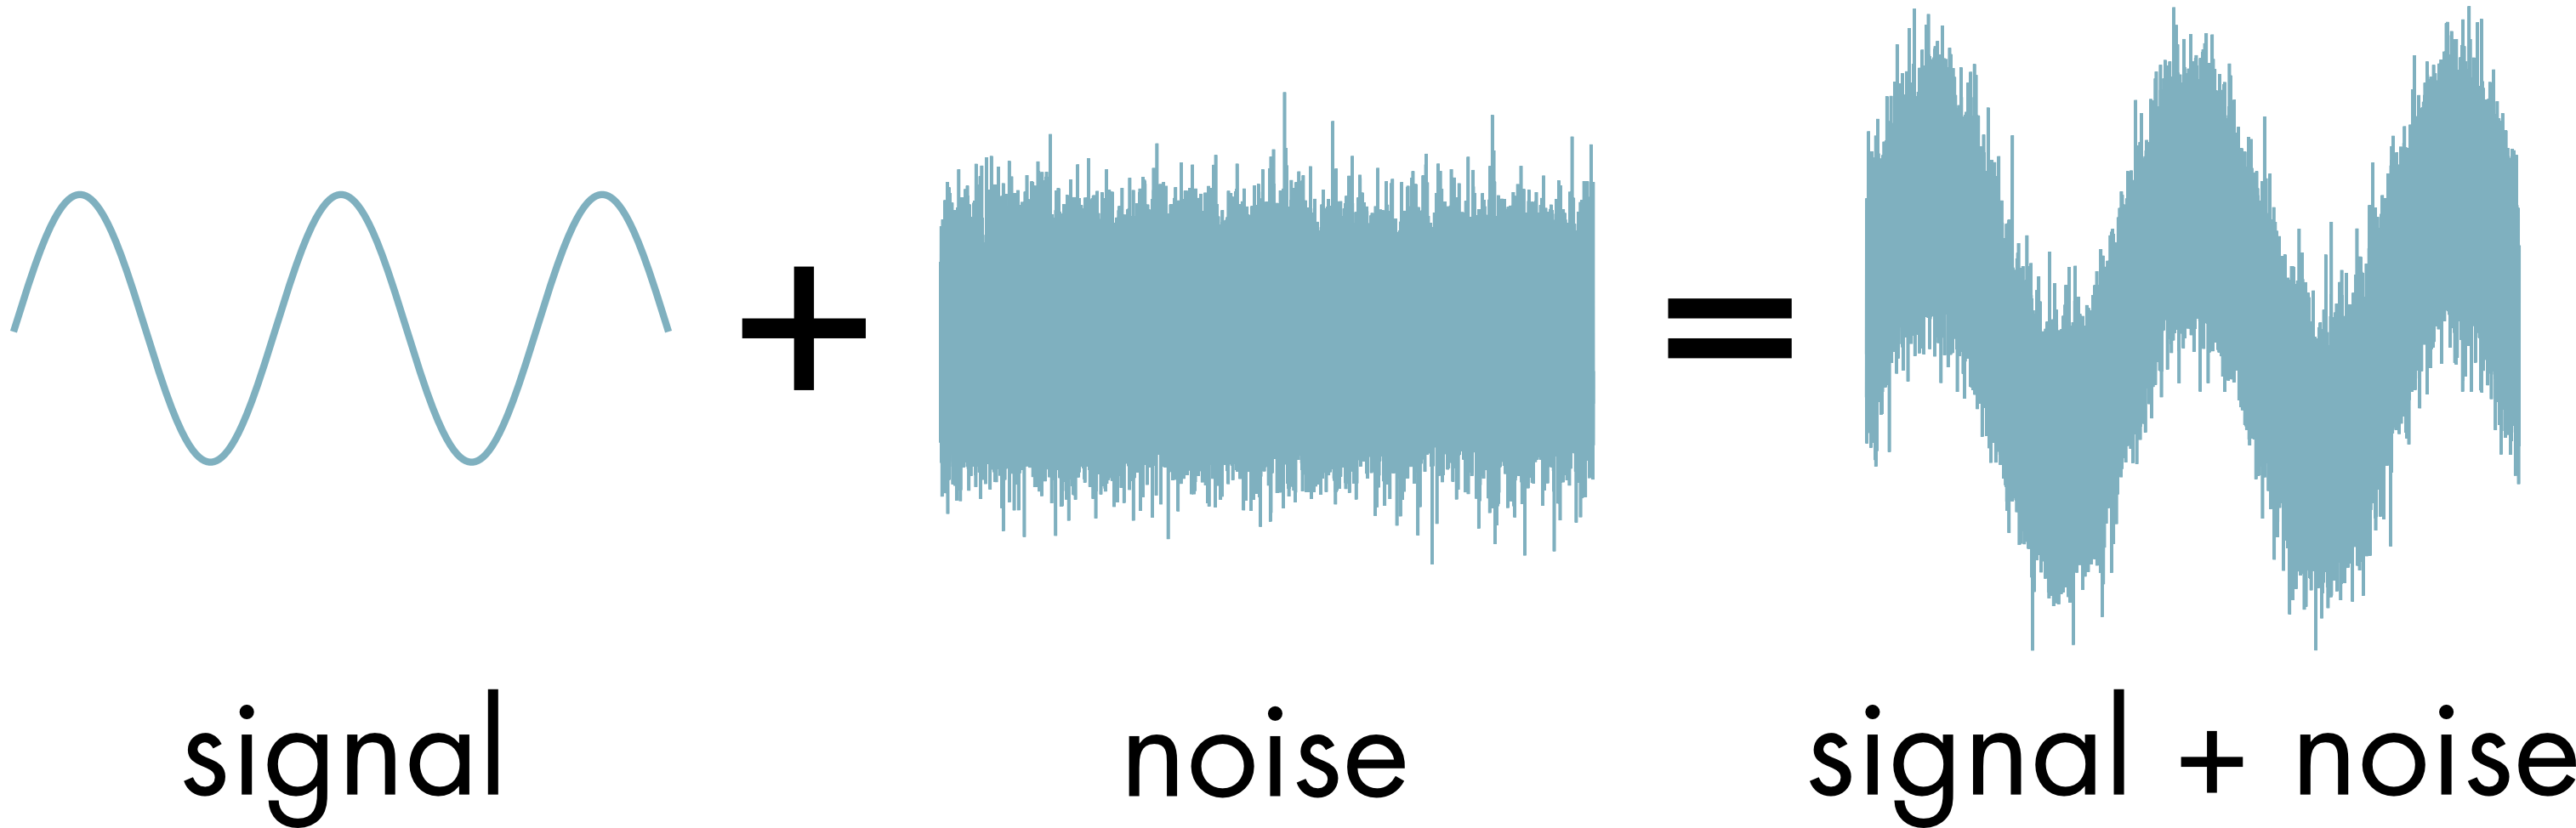
\includegraphics[width=\textwidth]{../images/s2n.png}
    \end{center}
    \alertGreen{Aspectos de modelamiento: superposición, filtro, etc}
\end{frame}
%%%%%%%%%%%%%%%%%%%%%%%%%%%%%%%%%%%%%%%%%%%%%%%%%%%%%%%
\begin{frame}{En el lenguaje de lo que conocemos}
    \begin{itemize}
        \item<+-> Una señal es una función $\to$ un punto de un espacio funcional
            $$ f(x) = \sin x $$
        \item<+-> Las señales se pueden superponer (suma!)
            $$ f_1(x)=\sin x, \quad f_2(x) = \cos x \quad \Rightarrow (f_1+f_2)(x) = \sin x + \cos x$$
        \item<+-> Las señales se pueden modular (producto por escalar!)
            $$ f(x) = \sin x \quad \Rightarrow (\alpha f)(x) = \alpha \sin x $$
    \end{itemize}
\end{frame}
%%%%%%%%%%%%%%%%%%%%%%%%%%%%%%%%%%%%%%%%%%%%%%%%%%%%%%%
\begin{frame}
    [VER EJEMPLOS DE SUMA Y PRODUCTO POR ESCALAR EN ESPACIO DE FUNCIONES]
\end{frame}
%%%%%%%%%%%%%%%%%%%%%%%%%%%%%%%%%%%%%%%%%%%%%%%%%%%%%%%
\begin{frame}{Espacios vectoriales}
    [DEFINIR INDEPENDENCIA LINEAL]
    [IDS TRIGONOMETRICAS CON DEPENDENCIA LINEAL]
\end{frame}
%%%%%%%%%%%%%%%%%%%%%%%%%%%%%%%%%%%%%%%%%%%%%%%%%%%%%%%
\begin{frame}{Espacios de Hilbert}
    [DEFINIR ESPACIO DE HILBERT]
    [VER EJEMPLO DE PROYECCION]
    [MOSTRAR SERIE TRUNCADA DE FUNCION ESCALON, HACERLO NUMERICO]
\end{frame}
%%%%%%%%%%%%%%%%%%%%%%%%%%%%%%%%%%%%%%%%%%%%%%%%%%%%%%%
\begin{frame}
    \maketitle
\end{frame}
%%%%%%%%%%%%%%%%%%%%%%%%%%%%%%%%%%%%%%%%%%%%%%%%%%%%%%%
\end{document}
